% --------------------------------------------------------------
% This is all preamble stuff that you don't have to worry about.
% Head down to where it says "Start here"
% --------------------------------------------------------------
 
\documentclass[12pt]{article}
 
\usepackage[margin=1in]{geometry} 
\usepackage{amsmath,amsthm,amssymb}
\usepackage{braket}
\usepackage{graphicx}
\usepackage{calligra}
\usepackage{calrsfs}
\usepackage{subcaption}
\usepackage{listings}
\newcommand{\N}{\mathbb{N}}
\newcommand{\Z}{\mathbb{Z}}
 
\newenvironment{theorem}[2][Theorem]{\begin{trivlist}
\item[\hskip \labelsep {\bfseries #1}\hskip \labelsep {\bfseries #2.}]}{\end{trivlist}}
\newenvironment{lemma}[2][Lemma]{\begin{trivlist}
\item[\hskip \labelsep {\bfseries #1}\hskip \labelsep {\bfseries #2.}]}{\end{trivlist}}
\newenvironment{exercise}[2][Exercise]{\begin{trivlist}
\item[\hskip \labelsep {\bfseries #1}\hskip \labelsep {\bfseries #2.}]}{\end{trivlist}}
\newenvironment{reflection}[2][Reflection]{\begin{trivlist}
\item[\hskip \labelsep {\bfseries #1}\hskip \labelsep {\bfseries #2.}]}{\end{trivlist}}
\newenvironment{proposition}[2][Proposition]{\begin{trivlist}
\item[\hskip \labelsep {\bfseries #1}\hskip \labelsep {\bfseries #2.}]}{\end{trivlist}}
\newenvironment{corollary}[2][Corollary]{\begin{trivlist}
\item[\hskip \labelsep {\bfseries #1}\hskip \labelsep {\bfseries #2.}]}{\end{trivlist}}
 
\begin{document}
 
% --------------------------------------------------------------
%                         Start here
% --------------------------------------------------------------
 
%\renewcommand{\qedsymbol}{\filledbox}
 
\title{HW7}
\author{Carl Mueller\\ %replace with your name
CSCI 5254 - Convex Optimization} %if necessary, replace with your course title
\maketitle

\subsection*{8.16}
Formulate the following asa CVX optimization problem:\\
Find the rectangle
$$R = \set{x \in \textbf{R}^n | l \preceq x \preceq u}$$
of maximum volume enclosed in the polyhedron
$$P = \set{x | Ax \preceq b}$$\\
The volume can be expressed as:
\begin{proposition}{1}
\begin{align}
v = \prod_{i=1}^{n}u_i-l_i
\end{align}
\end{proposition}
We want all the $2^n$ corners do be contained within the polyhedron. This every corner must meet the polyhedron constraint $Ac \preceq b$. Where $c$ is the vector of corners. Each of these corners can be be more succinctly represented as the vector based on the upper and lower values of each edge:\\ 
If we express $x_i$ as $u_i-l_i$ then this system becomes
$$\sum_{i=1}^{n}a_{ij}(u_j-l_j) \le b_i$$\\
The problem can be expressed as:
\begin{equation*}
\begin{aligned}
& \underset{}{\text{minimize}}
& & \prod_{i=1}^{n}u_i-l_i\\
& \text{subject to}\
& &\sum_{i=1}^{n}a_{ij}(u_j-l_j) \le b_i
\end{aligned}
\end{equation*}
The constraint is a posynomial as it is a summation of the monomial $a_{ij}(u_j-l_j)$.\\
To make the problem a non-linear geometric optimization problem, we take the log of the objective:
\begin{equation*}
\begin{aligned}
& \underset{}{\text{minimize}}
& & \sum_{i=1}^{n}log(u_i-l_i)\\
& \text{subject to}\
& &\sum_{i=1}^{n}a_{ij}(u_j-l_j) \le b_i
\end{aligned}
\end{equation*}

\subsection*{8.24}
We make use of the Cauchy-Schwarz inequality and sustite $p$ knowing that $||u||_2 \le p$:
\begin{proposition}{1}
\begin{align}
u^tx_i \le ||u||_2|x_i||_2\\
||u||_2||x_i||_2 \le p||x_i||_2\\
u^ty_j \le ||u||_2|y_j||_2\\
||u||_2|y_j||_2 \le p||y_j||_2\\
-||u||_2||y_j||_2 \ge -p||y_j||_2\\
\end{align}
\end{proposition}
For $x_i$:
\begin{equation*}
\begin{aligned}
(a+u)^Tx_i \ge b\\
a^Tx_i+u^Tx_i \ge b\\
a^Tx_i+||u||_2|x_i||_2 \ge b\\
a^Tx_i+p|x_i||_2 \ge b\\
a^Tx_i-b \ge -p|x_i||_2
\end{aligned}
\end{equation*}
For $x_i$:
\begin{equation*}
\begin{aligned}
(a+u)^Ty_j \le b\\
a^Ty_j+u^Ty_j \le b\\
a^Ty_j+||u||_2||y_j||_2 \le b\\
a^Ty_j+p||x_i||_2 \le b\\
a^Ty_j-b \le -p||y_j||_2\\
b-a^Ty_j \ge p||y_j||_2
\end{aligned}
\end{equation*}
The optimization problem:
\begin{equation*}
\begin{aligned}
& \underset{}{\text{minimize}}
& & p\\
& \text{subject to}\
& & b-a^Ty_j \ge p||y_j||_2\\
&&& a^Tx_i-b \ge -p|x_i||_2\\
&&& ||a||_2 \le 1
\end{aligned}
\end{equation*}\\
\textbf{Additional Exercises:}\\
\subsection*{5.12}
One heurisitc estiamte an initial $\hat{x}$ using the huber penalty function. We then use that $\hat{x}$ to estimate a $\hat{P}$ by aligning the indices of $Ax$ and $y$ to find a permutation matrix. Then using that same permutation we reoptimized for $\hat{x}$. We repeat this algorithm until the euclidean norm of the distance between the $\hat{x}_{\tau}$ and $\hat{x}_{\tau-1}$ is below some tolerance, $\tau$ being the current iteration step.

TODO CODE CODE AND EVALUATION

\subsection*{5.18}
We can reformulate the problem as the original object being less than or equal to some value $z$:
\begin{equation*}
\begin{aligned}
1+max_{k\neq y_i} f_k(x_i)  - f_{y_i} (x_i) \leq z_i,  z_i\geq 0\\
\end{aligned}
\end{equation*}\\
This can be represented by the following problem:
\begin{equation*}
\begin{aligned}
& \underset{}{\text{minimize}}
& &  \sum_i z_i + \mu ||A||_F^2\\
& \text{subject to}\
& & 1+max_{k\neq y_i} f_k(x_i) - f_{y_i} (x_i) \leq z_i, \forall i\\
&&&  1^T b= 0,   z \geq 0\\
\end{aligned}
\end{equation*}\\
This can be reexpressed using the individual inequality constraints:
\begin{equation*}
\begin{aligned}
& \underset{}{\text{minimize}}
& &  \sum_i z_i + \mu ||A||_F^2\\
& \text{subject to}\
& &  1^T b= 0,   z \geq 0\\
&&&  1+a_k^Tx_i + b  - y_i \leq z_i,    k = 1, 2, …,  y_i -1, y_i +1, …, K, i=1, 2, …, m
\end{aligned}
\end{equation*}\\
\begin{figure}[h]
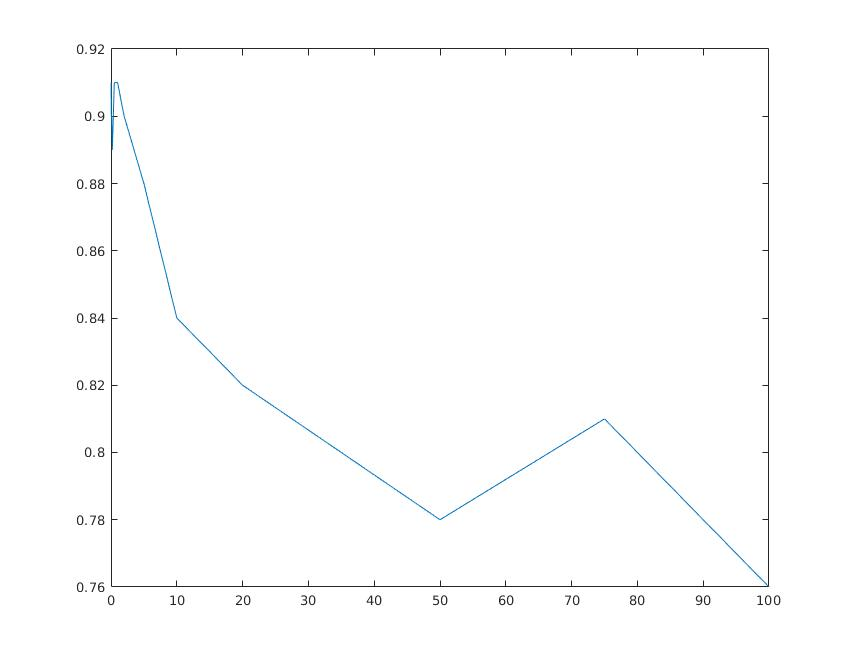
\includegraphics[scale=.25]{Problem_5_18.jpg}
\end{figure}
\textbf{Code:}\\
\begin{lstlisting}
E = [];
U = [0.01 0.05 0.1 0.2 0.5 1 2 5 10 20 50 75 100]
% This loop generates a new u value. 
for u = 1:size(U,2)
    cvx_begin
        variable z(mTrain, 1)
        variable A(K, n)
        variable b(K, 1)
        minimize(sum(z) + U(u)*square_pos(norm(A,'fro')))
        subject to
        for i=1:mTrain
            for k=[1:y(i)-1 y(i)+1:K]
                1+(A(k,:)*x(:,i)+b(k))-(A(y(i),:)*x(:,i)+b(y(i))) <= z(i);
            end
            z(i) >= 0;
        end
        sum(b) == 0;
    cvx_end
    % Compute the predict predicted labels by computing the affine function
    % on xtest using the estimated optial A and b. Find the max in each
    % column (i.e. argmax for label) and round to get whole number value.
    correct = 0
    y_pred = zeros(1,mTest);

    for i=1:mTest
        [~, y_pred(i)] = max(A*xtest(:,i) + b);
        if (y_pred(i) == ytest(i))
            correct = correct + 1;
        end
    end
    percent_correct = correct/mTest
    E = [E ; percent_correct]    
end
plot(U,E)
\end{lstlisting}


\subsection*{13.15}
One heurisitic is to ensure that the 1-norm of $w$ is minimized. We can then formulate and optimization problem subject to the following constraint:
\begin{proposition}{1}
\begin{align}
E[(r-\bar{r})((r-\bar{r})] = \Sigma\\
E[rr^T] - \bar{r}\bar{r}^T = \Sigma\\
E[rr^T] = \Sigma + \bar{r}\bar{r}^T
\end{align}
\end{proposition}
\begin{proposition}{2}
\begin{align}
E[z^Tz] = c^Tdiag(\Sigma) + \bar{r}^Tcc^T\bar{r}
\end{align}
\end{proposition}
\begin{equation*}
\begin{aligned}
E[(z-w^Tr)(z-w^Tr)] \le .01E[z^2]\\
E[z^Tz + r^Tww^Tr - 2zw^Tr ] \le .01E[z^2]\\
E[z^Tz] + E[r^Tww^Tr] - 2E[zw^Tr] \le .01E[z^2]\\
E[z^Tz] + E[r^Tww^Tr] - 2E[zw^Tr] \le .01E[z^2]\\
E[z^Tz] + E[w^Trr^Tw] - 2E[(c^Tr)^Tw^Tr] \le .01E[z^2]\\
c^Tdiag(\Sigma) + \bar{r}^Tcc^T\bar{r} + w^T(\Sigma + \bar{r}\bar{r}^T)w - 2E[(c^Tr)^Tw^Tr] \le .01E[z^2]\\
c^Tdiag(\Sigma) + \bar{r}^Tcc^T\bar{r} + w^T(\Sigma + \bar{r}\bar{r}^T)w - 2w^T(\Sigma + \bar{r}\bar{r}^T)c \le .01E[z^2]\\
\end{aligned}
\end{equation*}\\
This becomes the optimization problem reflected in the matlab code:
\begin{equation*}
\begin{aligned}
& \underset{}{\text{minimize}}
& &  ||w||_1\\
& \text{subject to}\
& & c^Tdiag(\Sigma) + \bar{r}^Tcc^T\bar{r} + w^T(\Sigma + \bar{r}\bar{r}^T)w - 2w^T(\Sigma + \bar{r}\bar{r}^T)c \le .01E[z^2]\\
\end{aligned}
\end{equation*}\\
\textbf{Code:}\\
\begin{lstlisting}
ctc = mtimes(c', c);
rbarsq = dot(rbar, rbar');
zsqr = (ctc * rbarsq)
cvx_begin
  variable w(n)
  minimize norm(w,1)
  E_num = ( (rbar' * (c * c') * rbar)) + c'*diag(Sigma) + (w' * (Sigma + (rbar * rbar')) * w) - 2 * w' *(Sigma + (rbar * rbar')) * c ;
  subject to
      E_num <= 0.01 * (ctc * rbarsq);
      w <= c;
cvx_end
E_num/(ctc * rbarsq)
sum(abs(w > 0.01))
sum(abs(c > 0.01))
\end{lstlisting}
\textbf{Results:}\\
ans = 0.0100\\
ans = 108\\
ans = 500\\

\subsection*{16.5}
See solution.

\subsection*{17.4}
\subsection*{17.5}
\subsection*{17.8}
\subsection*{17.9}
% --------------------------------------------------------------
%     You don't have to mess with anything below this line.
% --------------------------------------------------------------
 
\end{document}